\chapter{Introduction}
Embedded systems \parencite{leveson_embedded_2003} are special-purpose computer systems---composed of a processor, memory, software, and peripherals for input and ouput---that are embedded into a larger mechanical or electronic system.
Embedded systems are different from general-purpose computers such as desktops, laptops, mobile phones, and tablets because they typically run a single program which is tightly integrated to the accompanying hardware it is embedded within.
Their function is often to control or monitor a machine, which requires their program to react in real-time to sensor information or user input.

Arduino is a popular starting point for learning embedded systems today.
According to its \href{https://www.arduino.cc/en/Guide/Introduction}{official website}, 
``Arduino is an open-source electronics platform based on easy-to-use hardware and software'' \parencite{arduino_what_2018}.
It comprises of three main elements: 
hardware boards, the most famous of which is the Arduino Uno, shown in Fig.~\ref{fig:arduino_uno};
a microcontroller programming interface (API) and libraries in the C++ programming language, known as the \emph{Arduino language};
and an integrated development environment, the Arduino IDE.
Its low price, usability, and extensive community support make it an excelent entry point for learning embedded systems and an rapid prototyping tool for experts.

\begin{figure}[b]
  %\begin{wide}
    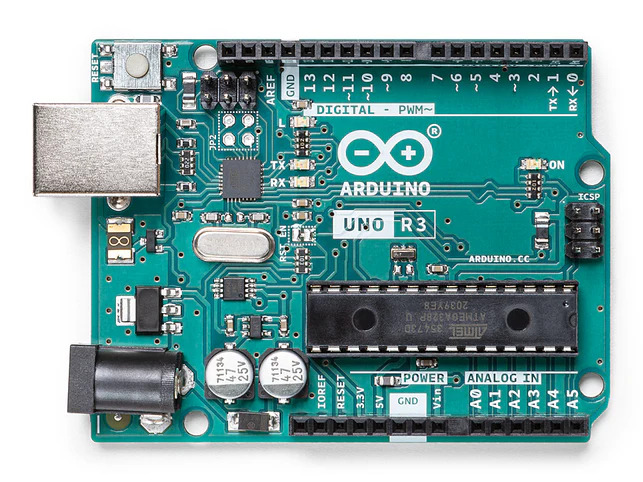
\includegraphics[width=0.5\textwidth]{img/arduino_uno_rev3}%
    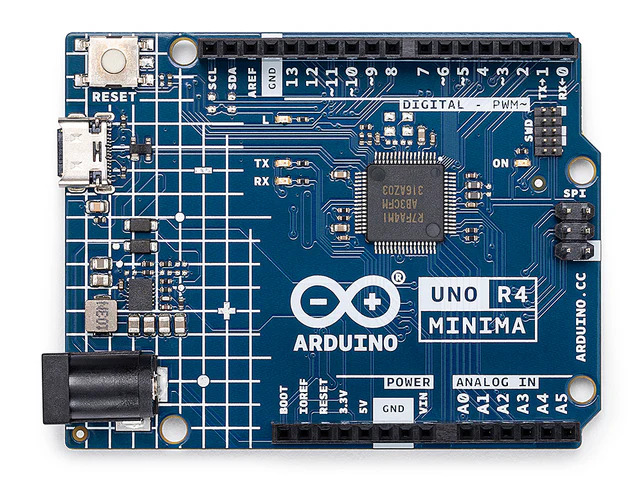
\includegraphics[width=0.5\textwidth]{img/arduino_uno_rev4}%
    \\ \scriptsize
    Source: \url{https://store.arduino.cc/collections/edu-boards}, under the \href{https://creativecommons.org/licenses/by-sa/3.0/legalcode}{Creative Commons Attribution ShareAlike 3.0} license.
    \caption{Arduino Uno Board Revisions R3 and R4 Minima.}
    \label{fig:arduino_uno}
  %\end{wide}
\end{figure}

This book is a introduction to embedded system programming with Arduino and C++.
Its main goal is laying out the foundations to understand the basic syntax of C++ and the while highlighting the unique aspects that distinguish embedded systems programming.
Its goal is enable readers to embed Arduinos or similar boards in their projects, leveraging existing libraries and frameworks instead of writing everything from scratch.
By understanding the core principles, readers will be able to integrate third-party code, modify existing solutions to fit their needs, build upon open-source projects, and even use AI in the software development process.
This approach also fosters good software engineering practices, such as code reuse, modular design, and systematic testing for robustness and correctness


\section{Platforms}
A defining characteristic of embedded systems is that the software is tightly coupled to the hardware it runs on.
Because of this, it is crucial to test your code on a physical hardware board to ensure proper functionality. Fortunately, many embedded platforms are affordable and widely available, making it easy to acquire a board for hands-on development.

Recommended boards for this book are:
\begin{description}
\item[Arduino Uno R3]
  The classic entry-level embedded platform, with many tutorials, example projects, libraries, drivers, and compatible hardware that snap in as Arduino Shields to extend its capabilities.
  However, in 2025 it sits on a akward spot of most expensive (around \SI{27}[\$]{}) and least capable of the boards in this list.
  With only \SI{2}{KB} of RAM, it does provide a great opportunity to learn how to manage constraints in embedded systems development.
  It is also a very forgiving board, robust against short-circuit, overvoltage, and general mishandling.
\item[Arduino Uno R4]
  A cheaper (around \SI{27}[\$]{}) and more capable version of the R3, the Uno R4 has better performance and more features while maintaining the same form factor and voltage levels.
  It offers improved processing power, more memory, and additional peripherals, making it suitable for a broader range of projects.
  An excellent choice if you need more capability than the R3 but still prefer to stick with the familiar Arduino environment.
\item[ESP32]
  A family of low-cost platforms, starting at below \SI{5}[\$]{}, that offer a lot of performance.
  All boards feature built-in wireless communication (Wi-Fi and Bluetooth) and dual-core processors.
  The ESP32 is a great choice for projects involving connectivity or real-time processing.
  It can be programmed in C/C++, Python, Lua, and other languages.
\item[Raspberry Pi Pico 2]
  A highly capable option, starting at around \SI{5}[\$]{}, with dual-core ARM architecture and ample memory.
  Offers wireless capabilities in some variants and is compatible with both C++ and MicroPython, making it suitable for a variety of coding environments.
  The Raspberry Pi Pico is particularly beneficial for users who want a small, affordable board with substantial memory and processing power.
\end{description}

Simulation can also be a valuable tool, especially in the early stages of development or when hardware is not immediately accessible.
Simulators allow you to prototype, debug, and test code without the need for physical deployment, though they may not always capture the full range of hardware interactions.
They are also often used in automated testing and continuous integration (CI), allowing developers to catch and fix bugs early.

Recommended simulation environments for this book are:
\begin{description}
\item[Wokwi] 
\item[TinkerCad] 
\end{description}

Most examples in this book can be done either in a hardware board or in simulation.
For best learning, however, familiarity with hardware is important.
Having a physical board on hand is also essential for using what you learn in personal, academic, and professional projects, beyond the book examples, which is the ultimate goal of the book.

\section{Hello World on the Wokwi Simulator}
The simplest way to get started with the Arduino, for the purpose of understanding the C++ language, is using the Wokwi online electronics simulator at \href{https://wokwi.com}{wokwi.com}.
To begin, open the Hello World program shown in 

\begin{figure}
  \begin{wide}
    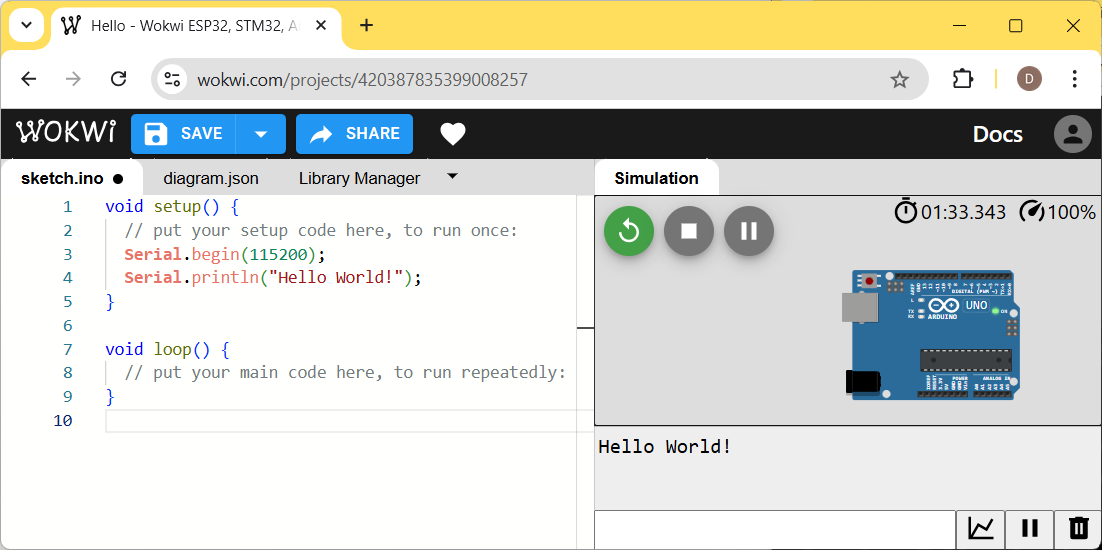
\includegraphics[width=\textwidth]{img/wokwi-hello.png}
    \\ \scriptsize
    Access this on \url{https://wokwi.com/projects/420387835399008257}
    \caption{Hello World program on the Wokwi simulator.}
    \label{fig:wokwi-hello}    
  \end{wide}
\end{figure}

%%% Local Variables:
%%% TeX-master: "main"
%%% eval: (adaptive-wrap-prefix-mode t)
%%% eval: (visual-line-mode t)
%%% eval: (nlinum-mode t)
%%% TeX-engine: luatex
%%% End:
